\glsreset{mypgd}
\glsreset{myholpgd}
To demonstrate applicability in a higher-dimensional setting, we consider a Bayesian image deblurring problem, following \cite{encinar2025proximal}. Here we are given an information-destroying blurring operator, $B$, acting on an image and the goal is to recover a latent clean image, $x\in\mathbb{R}^{d_x}$, from a noisy blurred observation $y=Bx^\star+\epsilon$ and ground-truth image $x^\star\in\mathbb{R}^{d_x}$. Applying the anisotropic \gls*{totalvariation} penalty, $p_\theta(x)=C^{-1}_\theta \exp(-e^{\theta}\mathrm{TV}(x))$ we have the posterior,
\begin{equation*}
    \pi_\theta(x)\propto \exp\left(-\frac{1}{2\sigma^2}\|y-Bx\|_2^2-e^\theta\mathrm{TV}(x)\right),
\end{equation*}
with the non-differentiable total variation $\mathrm{TV}(x):=\|\nabla_d x\|_1$ and $\nabla_d$ the two-dimensional discrete gradient operator. We additionally assume $C_\theta<\infty$ such that the prior is well-defined. Framed as the \gls*{mmle} of $p_\theta(y)$, we may write the loss function as in \eqref{eq:obj_func} with,
\begin{equation*}
    \nabla_\theta\ell(\theta)=\mathbb{E}_{X\sim\pi_\theta}\left[e^\theta\mathrm{TV}(X)-d_x\right].
\end{equation*}
Following \cite{encinar2025proximal} we use proximal techniques and \gls*{my} approximations to deal with the non-differentiability of the total variation, which we discuss in Appendix~\ref{app:mmle_details}. We compare the baseline \gls*{mypgd} with a higher-order Langevin scheme following the sampler dynamics introduced in \cite{high_order_langevin_JMLR}. Using gradient descent on the parameters we have the particle SDE:
\begin{equation}\label{eq:high_order_langevin_scheme}
    \begin{aligned}
        \md \theta_t&=-\frac{1}{N}\sum_{i=1}^NF(\theta_t,X^i_t)\md t,\\
        \md X^i_t&=U^i_t\md t,\\
        \md U^i_t&=-\nabla_xE^\lambda(\theta_t,X^i_t)\md t+\gamma V_t^i\md t,\\
        \md V^i_t&=-\gamma U^i_t\md t-\alpha V^i_t\md t+\sqrt{2\alpha}\md B^i_t,
    \end{aligned}
\end{equation}
where we note that we have $F(\theta,x)=\nabla_\theta E(\theta,x)$. We replace the non-differentiable $x$-gradient with $E^\lambda$, its \gls*{my} approximation, to obtain a hybrid proximal scheme, which we refer to as \gls*{myholpgd}. Both methods share the same optimiser dynamics but differ in the choice of Langevin scheme for the sampler dynamics.
\begin{figure}[t]
\centering
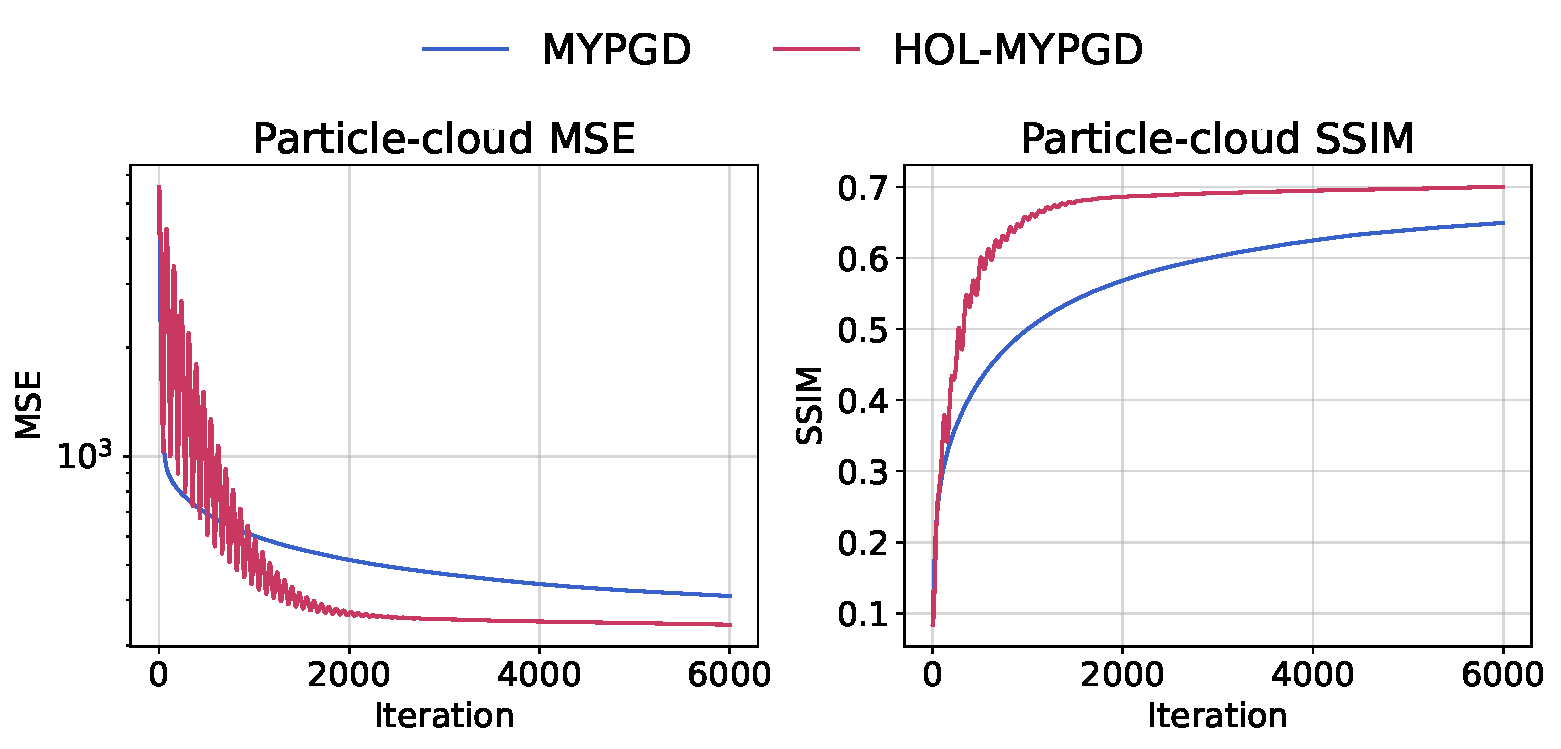
\includegraphics[width=0.7\textwidth]{images/mmle/mmle_deblurring_graphs_maintext.pdf} 
% one col: [width=0.7\textwidth]
% two col : [width=1.0\columnwidth]
\caption{Evolution of MSE (left) and SSIM (right) of the particle cloud mean across iterations, comparing methods \gls*{mypgd} and \gls*{myholpgd} for setup A.}
\label{fig:deblurring_example_graphs}
\end{figure}
We consider setups A and B with different blur and noise levels, providing full experimental details in Appendix~\ref{app:mmle_details}. Comparing MSE and SSIM between methods for setup A in Figure~\ref{fig:deblurring_example_graphs}, we find the high-order Langevin scheme converges faster and to more optimal values; other examples for setup B are given in the appendix. We also provide image reconstructions from particles in Figure~\ref{fig:deblurring_example} where we see \gls*{myholpgd} yields sharper reconstructions.

\begin{figure*}[ht]
    \centering
    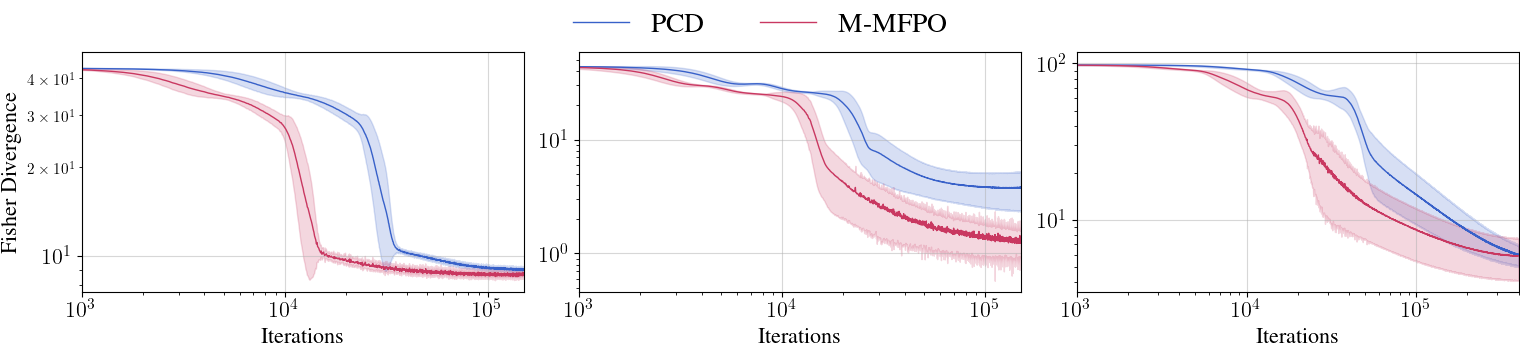
\includegraphics[width=1.0\textwidth]{images/main/final_comparisons.png}
    \caption{Comparison of Fisher divergence over iterations for the \textit{rings} (left), \textit{beads} (middle), and \textit{lattice} (right) datasets for \gls*{pcd} and \gls*{mmfpo} methods with $N=10,000$ particles. Curves show the mean across 25 independent runs, with shaded bands indicating ±1 standard deviations.}
    \label{fig:training_comparisons}
\end{figure*}